%----------------------------------------------------------------------------------------
%    PACKAGES AND THEMES
%----------------------------------------------------------------------------------------

\documentclass[aspectratio=169,xcolor=dvipsnames]{beamer}
\usetheme{SimplePlus}

\usepackage{tikz}
\usepackage{hyperref}
\usepackage{graphicx} % Allows including images
\usepackage{booktabs} % Allows the use of \toprule, \midrule and \bottomrule in tables
\usepackage{wrapfig}
\usepackage{listings}
\usepackage[font=small,labelfont=bf]{caption}

%----------------------------------------------------------------------------------------
%    TITLE PAGE
%----------------------------------------------------------------------------------------

\title{Unsupervised Learning}
\subtitle{HI 743}

\author{Ryan Gallagher}

\institute
{
    Department of Health Informatics and Administration \\
    Zilber College of Public Health \\
    University of Wisconsin - Milwaukee% Your institution for the title page
}
\date{March 25th, 2025} % Date, can be changed to a custom date


%----------------------------------------------------------------------------------------
%    PRESENTATION SLIDES
%----------------------------------------------------------------------------------------

\begin{document}
\begin{frame}
    % Print the title page as the first slide
    \titlepage
\end{frame}

%----------------------------------------------------------------------------------------
%    Outline
%----------------------------------------------------------------------------------------

\begin{frame}{Overview}
    % Throughout your presentation, if you choose to use \section{} and \subsection{} commands, these will automatically be printed on this slide as an overview of your presentation
    \tableofcontents
\end{frame}

%----------------------------------------------------------------------------------------
%    Slides
%----------------------------------------------------------------------------------------
\section{Review Final Project Rubric}
\begin{frame}{Title}
\centering
\textbf{Let's look at Final Project.pdf}
\end{frame}
%----------------------------------------------------------------------------------------


\section{Overview}
\begin{frame}{Unsupervised Learning}
  \textbf{What is Unsupervised Learning?}
  \begin{itemize}
    \item In supervised learning, we observe features $X_1, X_2, \ldots, X_p$ and a response $Y$, and our goal is to predict $Y$ using the $X$'s.
    \item In \textbf{unsupervised learning}, we only observe features $X_1, X_2, \ldots, X_p$—\emph{no response variable} $Y$.
    \item The goal is not prediction, but \textbf{exploration}: to discover interesting patterns or structures in the data.
  \end{itemize}

  \vspace{0.3cm}
  \textbf{Key Questions:}
  \begin{itemize}
    \item Is there a useful way to \textbf{visualize} the data?
    \item Can we identify \textbf{groups of similar observations or variables}?
  \end{itemize}

\end{frame}

\begin{frame}{Challenges of Unsupervised Learning}
  \textbf{"Exploratory Data Analysis" - Inference is Subjective}
  \begin{itemize}
    \item In supervised learning, model performance can be evaluated using $Y$
    \item In unsupervised learning, there is no obvious way to check if results are “correct”
  \end{itemize}

  \vspace{0.2cm}
  \textbf{Implications:}
  \begin{itemize}
    \item Many different valid ways to define structure or clusters
    \item Results depend heavily on:
    \begin{itemize}
      \item Method used
      \item Distance or similarity metrics
      \item Data scaling and preprocessing
    \end{itemize}
  \end{itemize}

  \vspace{0.3cm}
  \textit{Requires careful interpretation and domain knowledge}
\end{frame}

\section{Principal Component Analysis (PCA)}
\begin{frame}{Principal Component Analysis (PCA)}
  \textbf{What is PCA?}
  \begin{itemize}
    \item A method to reduce the dimensionality of a dataset.
    \item Finds new features (called \textbf{principal components}) that are:
    \begin{itemize}
      \item Linear combinations of the original variables.
      \item Uncorrelated with each other.
      \item Ranked by how much variance they explain in the data.
    \end{itemize}
    \item Often used for:
    \begin{itemize}
      \item Visualization of high-dimensional data.
      \item Preprocessing before supervised learning.
    \end{itemize}
  \end{itemize}

\end{frame}

\begin{frame}{What is a Principal Component?}
  \textbf{Definition:}
  \begin{itemize}
    \item A \textbf{principal component (PC)} is a direction in feature space along which the data varies the most.
    \item The first PC is the direction of \textbf{maximum variance}.
    \item The second PC is orthogonal to the first and explains the next highest variance, and so on.
  \end{itemize}

  \vspace{0.2cm}
  \textbf{Mathematically:}
  \begin{itemize}
    \item PC$_1$ = direction $v_1$ such that
    \[
    v_1 = \arg\max_{\|v\| = 1} \text{Var}(Xv)
    \]
    \item The projection of each observation onto $v_1$ gives the first principal component score.
  \end{itemize}
\end{frame}

\subsection{USArrests Data}
\begin{frame}{Visualizing PCA - USArrests}
  \begin{columns}
    \column{0.55\textwidth}
    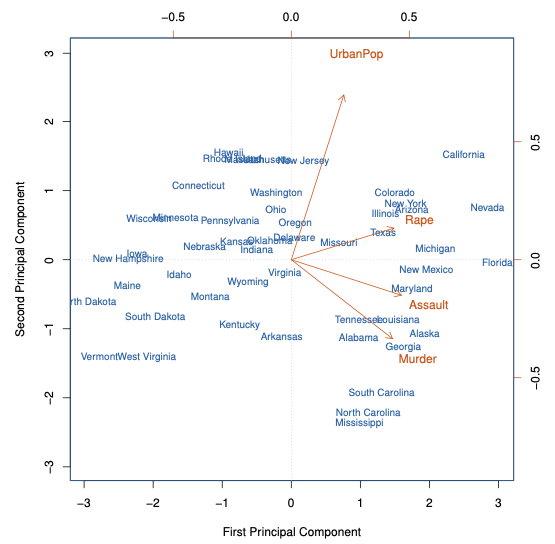
\includegraphics[width=\linewidth]{images/figure12_1.png} % Replace with actual path if available

    \column{0.4\textwidth}
    \textbf{USArrests data:}
    \begin{itemize}
      \item Data points in 2D (e.g., $X_1$ and $X_2$)
      \item \textbf{First Principal Component (PC1)}: direction of greatest variance
      \item \textbf{Second Principal Component (PC2)}: orthogonal to PC1, captures remaining variance
    \end{itemize}

    \vspace{0.3cm}
  \end{columns}
\end{frame}

\begin{frame}{PCA on USArrests Data (Figure 12.1)}
  \textbf{Context:}
  \begin{itemize}
    \item Dataset: \texttt{USArrests} — crime statistics (Murder, Assault, UrbanPop, Rape) for 50 U.S. states
    \item PCA applied after standardizing the variables
  \end{itemize}

  \vspace{0.3cm}
  \textbf{Results shown in Figure 12.1:}
  \begin{itemize}
    \item \textbf{PC1} accounts for the largest variance:
    \begin{itemize}
      \item Separates states with high rates of violent crimes (Murder, Assault, Rape)
    \end{itemize}
    \item \textbf{PC2} captures variation more related to UrbanPop
    \item States like California and Florida have high PC1 scores — indicating higher crime rates
  \end{itemize}

  \vspace{0.3cm}
  \textit{PCA reveals underlying structure: crime-heavy vs. low-crime states in fewer dimensions.}
\end{frame}

\begin{frame}{PCA Loadings: Table 12.1}
  \begin{columns}
    \column{0.55\textwidth}
    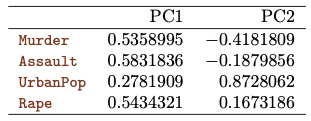
\includegraphics[width=\linewidth]{images/table12_1.png} % Ensure this file is in your project folder

    \column{0.42\textwidth}
    \textbf{Loadings}
    \begin{itemize}
      \item Loadings are coefficients that define each principal component.
      \item PC$_1$ emphasizes \texttt{Murder}, \texttt{Assault}, and \texttt{Rape}.
      \item PC$_2$ loads strongly on \texttt{UrbanPop} and contrasts with \texttt{Rape}.
    \end{itemize}
    
  \end{columns}
\end{frame}

\begin{frame}{Proportion of Variance Explained (PVE)}
  \textbf{PVE}
  \begin{itemize}
    \item Each principal component captures a different “direction” of variation in the data.
    \item PCA ranks these directions from most to least variation.
    \item The Proportion of Variance Explained (PVE) tells us how much of the total variation is captured by each component.
  \end{itemize}

  \vspace{0.3cm}
  \textbf{What insight does it give?}
  \begin{itemize}
    \item It helps us understand which components are most important for representing the data.
    \item A high PVE for the first few components means the data can be summarized well with fewer dimensions.
    \item PVE is typically visualized using a scree plot: a chart showing how much variation each component explains.
  \end{itemize}
\end{frame}

\section{Missing Values \& Matrix Completion}
\begin{frame}{Missing Values and Matrix Completion}
  \textbf{Missing Data} is common. In many datasets, some entries are missing. This is especially challenging in unsupervised settings where no outcome $Y$ is available to help fill in the blanks.


  \vspace{1cm}
  \textbf{Matrix Completion:}
  \begin{itemize}
    \item Unsupervised learning can estimate missing values using the observed data.
    \item It assumes the true data matrix has some underlying structure (e.g., low-rank).
    \item Common in recommendation systems (e.g., Netflix: users rate only a few movies).
  \end{itemize}
  \end{frame}

\begin{frame}{Fill in Missing Values via PCA (Algorithm 12.1)}
  \textbf{Goal:} Estimate the missing entries in a data matrix using the observed ones.

  \vspace{0.3cm}
  \textbf{Idea Behind the Algorithm:}
  \begin{itemize}
    \item We assume the complete data lies close to a low-dimensional space (like in PCA).
    \item Even with missing values, we can iteratively estimate the full matrix.
  \end{itemize}

  \vspace{0.3cm}
  \textbf{How It Works — In Plain Terms:}
  \begin{enumerate}
    \item \textbf{Start by filling in} the missing values with simple guesses (like column means).
    \item \textbf{Apply PCA} to the filled-in matrix to find the best low-rank approximation.
    \item \textbf{Replace the missing entries} with the values predicted by the PCA.
    \item \textbf{Repeat} until the estimates stop changing much.
  \end{enumerate}
\end{frame}

\begin{frame}{Figure 12.5: Matrix Completion with PCA}
  \begin{columns}
    \column{0.55\textwidth}
    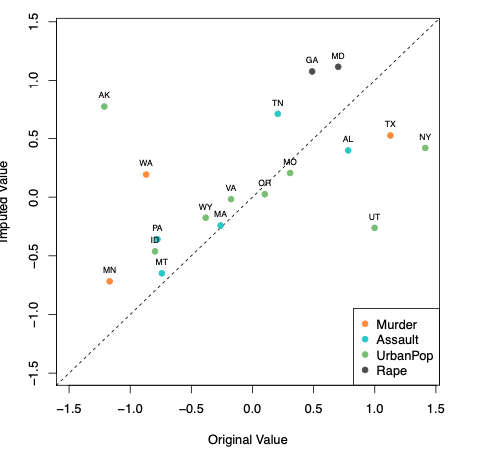
\includegraphics[width=\linewidth]{images/figure12_5.png} % Ensure this image is in your project folder

    \column{0.4\textwidth}
    \begin{itemize}
      \item Plot of the \texttt{USArrests} dataset with some values removed at random.
      \item Missing values were filled using PCA-based matrix completion.
      \item X \& Y axis agreement show accurate fit
    \end{itemize}
  \end{columns}
\end{frame}

\begin{frame}{K-Means Clustering - Quick Review}
 Group observations into $K$ distinct, non-overlapping clusters based on similarity.

  \vspace{0.3cm}
  \textbf{Algorithm}
  \begin{enumerate}
    \item Choose the number of clusters, $K$.
    \item Randomly assign each observation to one of the $K$ clusters.
    \item Compute the center (mean) of each cluster.
    \item Reassign observations to the nearest cluster center.
    \item Repeat steps 3–4 until assignments stop changing.
  \end{enumerate}

  \vspace{0.3cm}
  \textbf{Key Idea:} 
  \begin{itemize}
    \item Each cluster groups together observations that are close in terms of their features.
    \item The algorithm tries to minimize the variation within clusters.
  \end{itemize}
\end{frame}

\begin{frame}{Figure 12.8: K-Means Clustering}
  \begin{columns}
    \column{0.55\textwidth}
    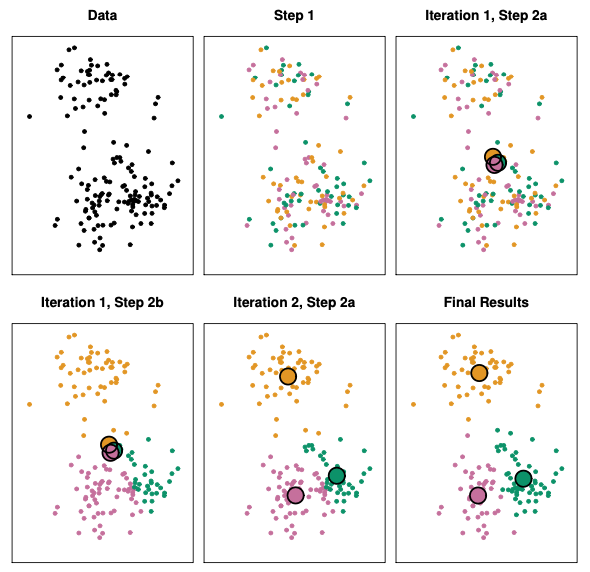
\includegraphics[width=\linewidth]{images/figure12_8.png} % Make sure this file is in your folder

    \column{0.42\textwidth}
    \begin{itemize}
      \item A toy dataset in two dimensions.
      \item Points are grouped into three clusters using K-means.
      \item Shows steps toward achieving the clustering.
      \item Each point is colored by its assigned cluster.
    \end{itemize}

  \end{columns}
\end{frame}


\begin{frame}{Hierarchical Clustering}
  \textbf{Concept Overview}
  \begin{itemize}
    \item Hierarchical clustering groups similar observations based on their distance.
    \item It creates a tree-like structure called a \textbf{dendrogram}, which shows how clusters are merged at different levels.
    \item Observations that are more similar are combined earlier (lower in the tree).
    \item Unlike K-means, you do not need to specify the number of clusters in advance.
  \end{itemize}

  \vspace{0.4cm}
  \textbf{The Algorithm (Produce a Dendrogram)}
  \begin{enumerate}
    \item Start with each observation in its own cluster.
    \item Compute the distances between all pairs of clusters.
    \item Merge the two clusters that are closest together.
    \item Repeat steps 2–3 until all observations are merged into a single cluster.
  \end{enumerate}
\end{frame}


\begin{frame}{Hierarchical Clustering: Building a Tree of Similarity}
  \begin{columns}
    \column{0.48\textwidth}
    \textbf{Concept Overview}
    \begin{itemize}
      \item Groups similar observations based on a notion of distance or similarity.
      \item Builds a tree-like structure called a \textbf{dendrogram}.
      \item Observations that are more similar are joined earlier in the tree.
    \end{itemize}

    \vspace{0.3cm}
    \textbf{Why Use It?}
    \begin{itemize}
      \item No need to choose the number of clusters in advance.
      \item Helps visualize nested groupings and relationships.
    \end{itemize}

    \column{0.48\textwidth}

    \vspace{0.3cm}
    \textbf{Cutting the Dendrogram}
    \begin{itemize}
      \item By slicing the dendrogram at a chosen height, you can form distinct clusters.
    \end{itemize}
  \end{columns}

  \vspace{0.4cm}
  \centering
  \textit{Hierarchical clustering reveals the structure of similarity in your data at multiple levels.}
\end{frame}


\begin{frame}{Figure 12.11: Cutting a Dendrogram for Clusters}
  \begin{columns}
    \column{0.55\textwidth}
    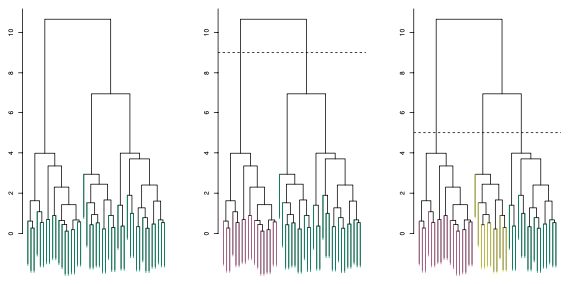
\includegraphics[width=\linewidth]{images/figure12_11.png} % Save and include this image from ISLR2

    \column{0.42\textwidth}
    \begin{itemize}
      \item \textbf{Left:} Full dendrogram from hierarchical clustering (complete linkage, Euclidean distance).
      \item \textbf{Center:} Cutting at height 9 forms \textbf{two clusters}.
      \item \textbf{Right:} Cutting at height 5 forms \textbf{three clusters}.
    \end{itemize}

    \vspace{0.2cm}

    \begin{itemize}
      \item The \textbf{height of the cut} determines the number of clusters.
      \item One dendrogram allows us to explore multiple clustering solutions.
    \end{itemize}
  \end{columns}

\end{frame}

\begin{frame}{Figure 12.12: Interpreting Dendrogram Structure}
  \begin{columns}
    \column{0.55\textwidth}
    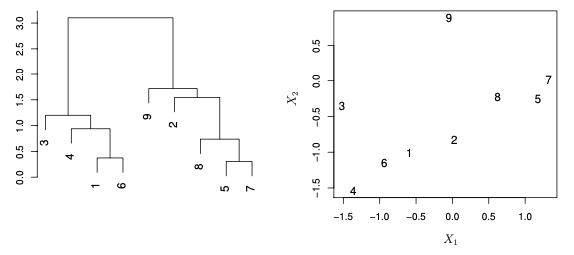
\includegraphics[width=\linewidth]{images/figure12_12.png} % Save this figure as a PNG and include it here

    \column{0.4\textwidth}
    \begin{itemize}
      \item \textbf{Left panel:} A dendrogram built from 9 observations using complete linkage.
      \item \textbf{Right panel:} The raw data used to generate the dendrogram, shown in 2D space.
      \item For example, observations 9 and 2 appear near each other, but are not more similar than 9 is to 5, 7, or 8.
    \end{itemize}
  \end{columns}
\end{frame}

\begin{frame}{Practical Issues: Scaling and Setup Choices}
  \textbf{Clustering isn't automatic — small choices can matter a lot.}

  \vspace{0.3cm}
  \textbf{Decisions that affect results:}
  \begin{itemize}
    \item \textbf{Should the variables be standardized?}
    \begin{itemize}
      \item Variables with larger scales (e.g., annual sock purchases vs. laptops) can dominate distance calculations.
      \item Scaling to standard deviation 1 gives each variable equal weight.
    \end{itemize}

    \item \textbf{Hierarchical Clustering Choices:}
    \begin{itemize}
      \item What dissimilarity measure should we use? (e.g., Euclidean, correlation)
      \item What type of linkage? (e.g., complete, average, single)
      \item Where should we cut the dendrogram?
    \end{itemize}

    \item \textbf{K-means Choices:}
    \begin{itemize}
      \item How many clusters ($K$) should we choose?
    \end{itemize}
  \end{itemize}
\end{frame}

\begin{frame}{Practical Issues: Validating and Interpreting}
  \textbf{Are the clusters meaningful? Or just random patterns?}

  \vspace{0.3cm}
  \textbf{Validating the Clusters Obtained:}
  \begin{itemize}
    \item Clustering methods \textit{will} produce groups—even from random data.
    \item We must ask: are these clusters real or noise?
    \item One approach: apply clustering to a dataset with no actual group structure (e.g., data drawn from a single Gaussian) and compare results.
  \end{itemize}

  \vspace{0.3cm}
  \textbf{Other Considerations:}
  \begin{itemize}
    \item Cluster analysis is more about \textbf{exploration} than strict inference.
    \item Results may depend heavily on:
    \begin{itemize}
      \item Method used (e.g., K-means vs. hierarchical)
      \item Distance metric
      \item Preprocessing choices (e.g., scaling)
    \end{itemize}
    \item It's common to try multiple methods and compare for robustness and interpretability.
  \end{itemize}
\end{frame}

\end{document}